% ==============================================================================
% CAPÍTULO 6: ESTUDIO COMPARATIVO DE RÉGIMEN: PROTONES VS. ELECTRONES
% ==============================================================================
\chapter{Estudio Comparativo de Régimen: Protones vs. Electrones Relativistas}

\section{Diferencias de Masa y Dinámica Relativista}
La física de aceleradores impone requerimientos geométricos opuestos según la masa en reposo de la partícula inyectada. Mientras que el protón posee una masa en reposo de $m_{0,p}c^2 = 938.272\text{ MeV}$, el electrón es una partícula ligera con $m_{0,e}c^2 = 0.511\text{ MeV}$.

Para una energía cinética inicial de $T_0 = 10.0\text{ MeV}$:
\begin{itemize}
    \item \textbf{Protón:} El factor relativista es $\gamma_p = 1.0107$ y su velocidad es $\beta_p = 0.1448$. Opera en un régimen no relativista ($\beta \ll 1$), donde la velocidad aumenta fuertemente con la energía ($\beta \propto \sqrt{T}$).
    \item \textbf{Electrón:} El factor relativista alcanza $\gamma_e = 20.57$ y su velocidad es $\beta_e = 0.9988 \approx 1.0$. El electrón es ultrarelativista desde la inyección, viajando casi a la velocidad de la luz.
\end{itemize}

\section{Congelamiento de Fase y Celdas de Longitud Constante}
Dado que los electrones adquieren $\beta \approx 1.0$ a bajas energías, la velocidad de la partícula no cambia perceptiblemente ante ganancias adicionales de energía cinética. En consecuencia, la condición de sincronismo para electrones no requiere celdas en expansión ($L_n = \beta_n \lambda$), sino una estructura resonante periódica con celdas de longitud constante:
\begin{equation}
L_e = \lambda = \frac{c}{f_{\text{RF}}} \approx 0.8512\text{ m}
\end{equation}

\begin{figure}[H]
    \centering
    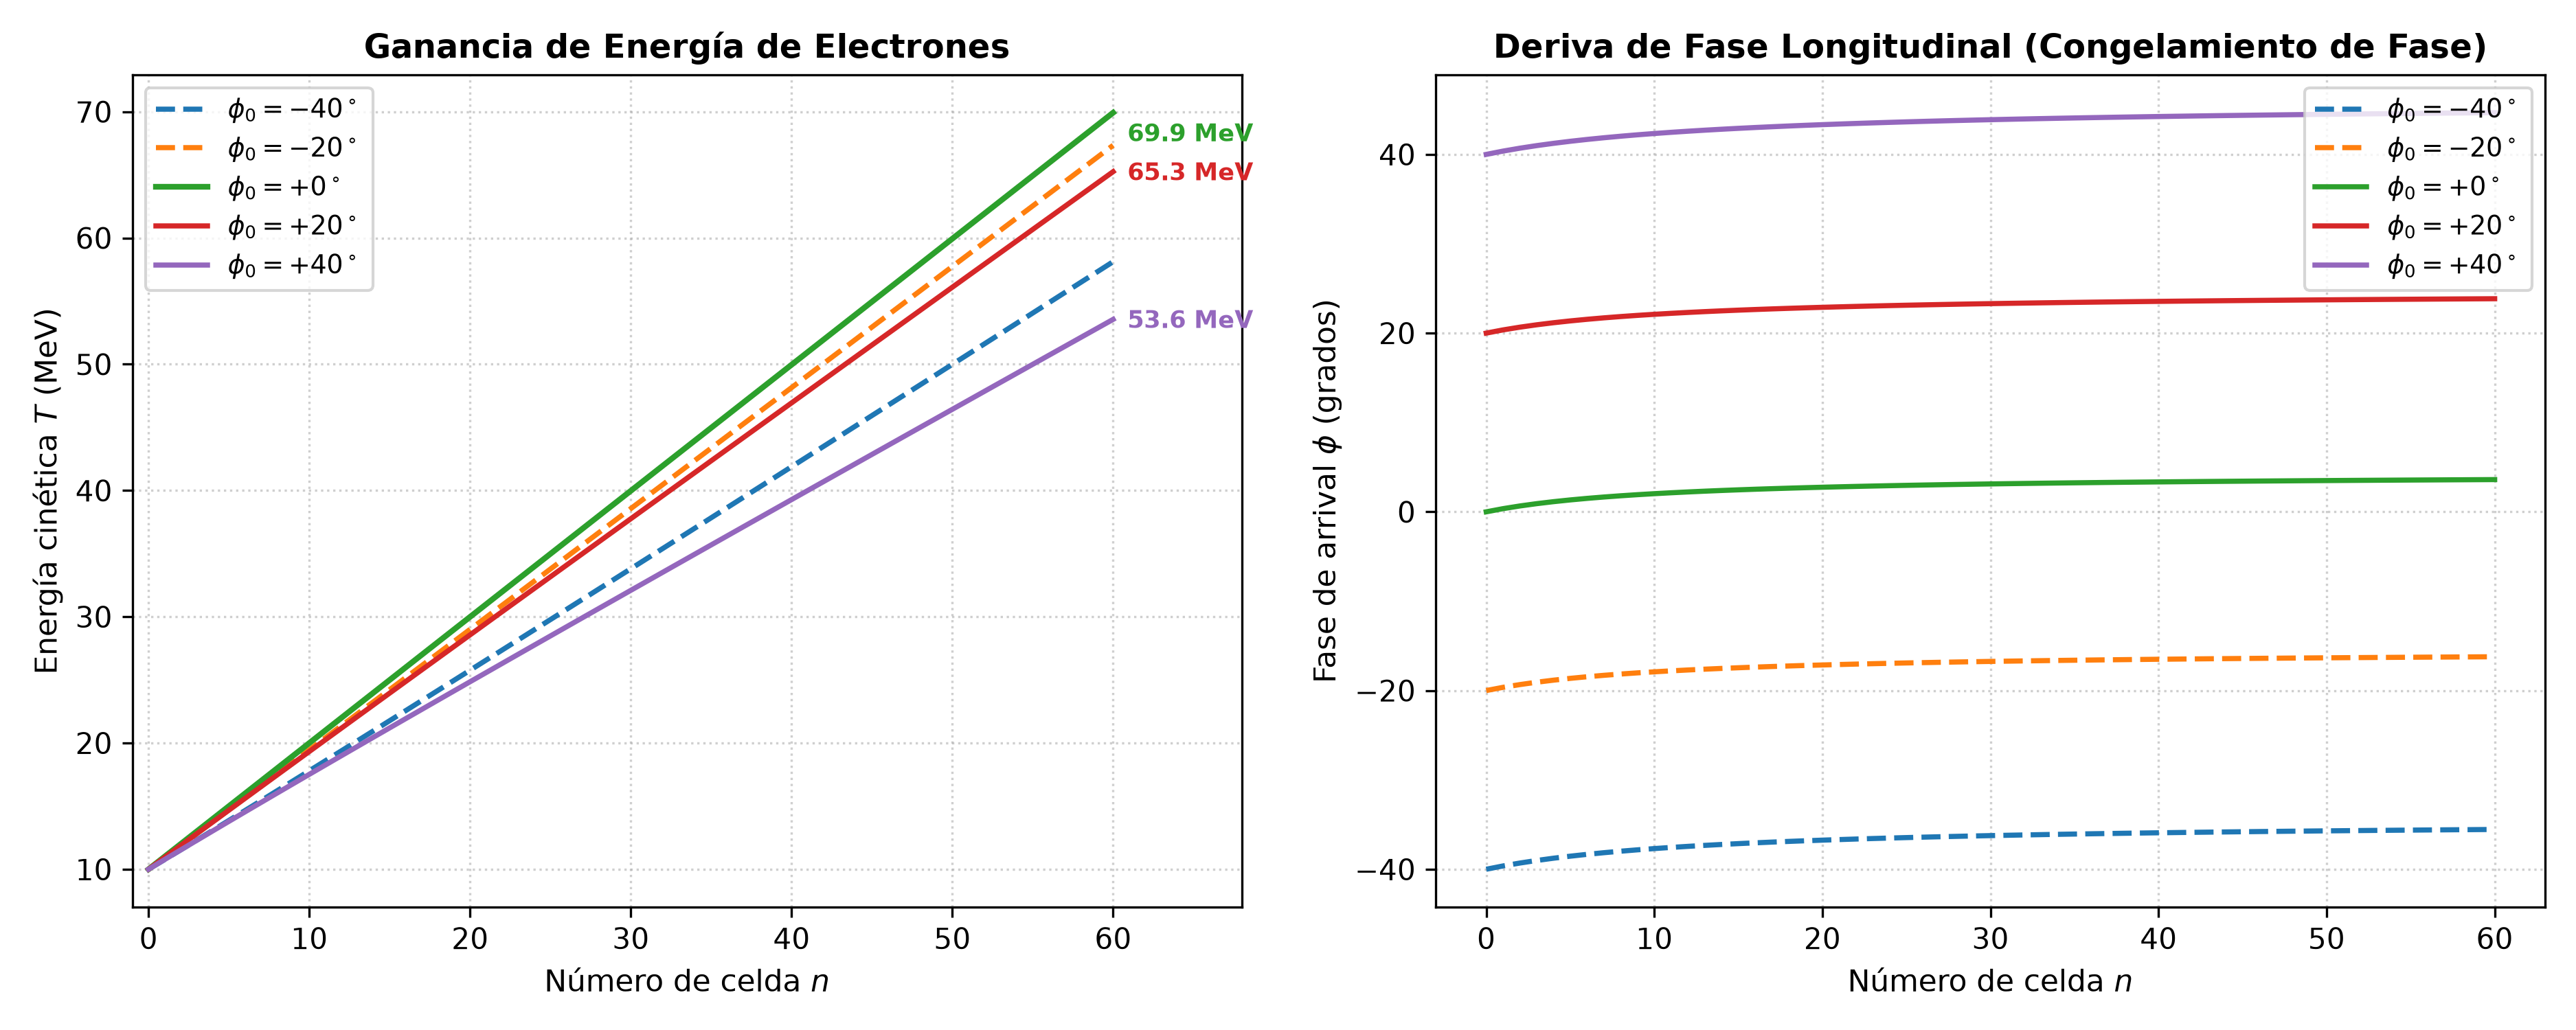
\includegraphics[width=0.85\textwidth]{figuras/fig05_estabilidad_electrones.png}
    \caption{Dinámica relativista de electrones en 60 celdas de longitud constante ($L = \lambda$): rápida saturación de $\beta \to 1.0$ (panel superior) y congelamiento de la fase de RF $\phi \to 0^\circ$ (panel inferior).}
    \label{fig:estabilidad_electrones}
\end{figure}

Como se ilustra en la Figura \ref{fig:estabilidad_electrones}:
\begin{enumerate}
    \item La velocidad adimensional $\beta_e$ permanece fija en $0.9988$, eliminando la necesidad de reestructurar la geometría de los tubos de deriva.
    \item La fase relativa de RF $\phi$ sufre un \textit{congelamiento de fase} acelerado, estabilizándose en $\phi \to 0^\circ$. Esto permite inyectar el haz en la cresta de máxima aceleración del campo electromagnético ($\cos 0^\circ = 1.0$).
\end{enumerate}

\section{Comparación de la Eficiencia Espacial de Aceleración (\texorpdfstring{$dT/dz$}{dT/dz})}
Una consecuencia fundamental del régimen cinemático es la tasa de ganancia energética por unidad de longitud ($dT/dz$ en $\text{MeV/m}$). 

\begin{figure}[H]
    \centering
    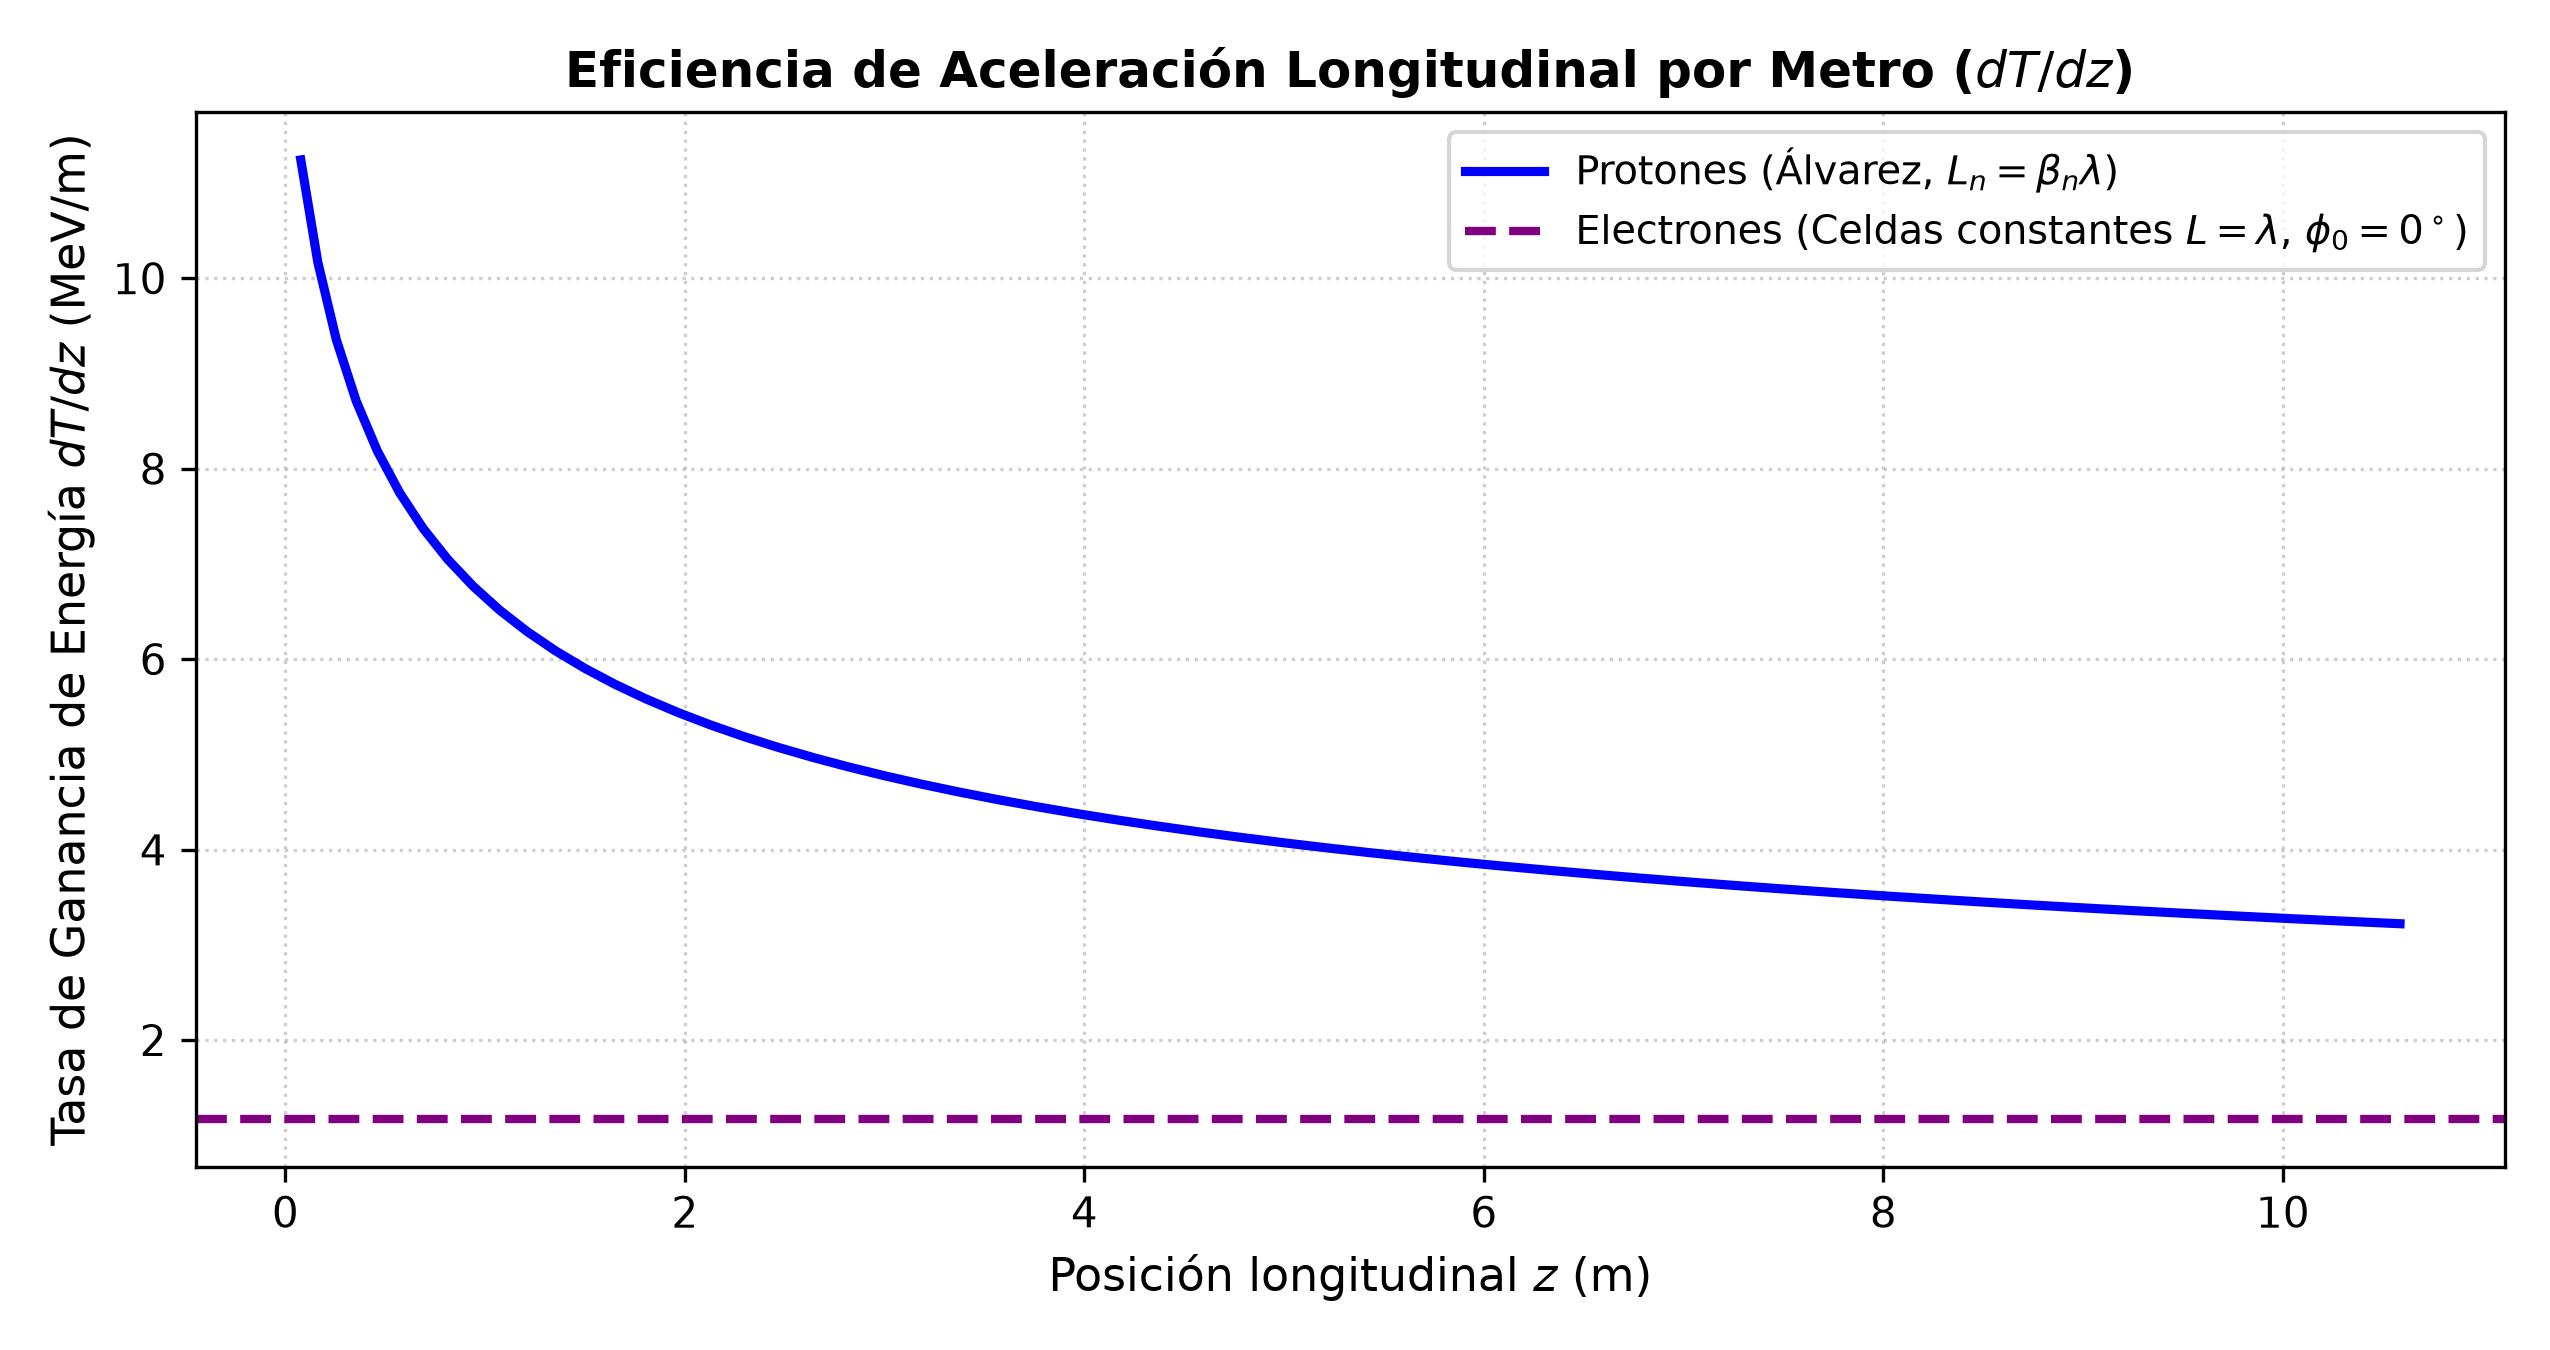
\includegraphics[width=0.85\textwidth]{figuras/fig09_tasa_ganancia_energia.png}
    \caption{Comparación de la tasa de ganancia de energía por metro ($dT/dz$) entre la estructura Álvarez para protones ($L_n = \beta_n \lambda$) y la estructura de celdas constantes para electrones ($L = \lambda$).}
    \label{fig:tasa_ganancia}
\end{figure}

La Figura \ref{fig:tasa_ganancia} evidencia el contraste operacional entre ambas estructuras:
\begin{itemize}
    \item \textbf{Protones (Estructura Álvarez):} Al inicio ($z < 1\text{ m}$), las celdas son breves ($L_1 = 7.70\text{ cm}$), ofreciendo una alta eficiencia espacial inicial de $dT/dz = 11.24\text{ MeV/m}$. A medida que las celdas se expanden hasta $26.89\text{ cm}$, la densidad de ganancia por metro cae en un $71.3\%$, estabilizándose en $3.22\text{ MeV/m}$.
    \item \textbf{Electrones (Celdas Constantes):} Debido a la constancia geométrica $L = 0.8512\text{ m}$ y al congelamiento de fase en la cresta ($\phi \to 0^\circ$), la tasa de aceleración espacial es estrictamente constante a lo largo de toda la cavidad:
    \begin{equation}
    \frac{dT}{dz} = \frac{q V_{\text{gap}} \cos(0^\circ)}{\lambda} = \frac{1.0\text{ MV}}{0.8512\text{ m}} \approx 1.1748\text{ MeV/m}
    \end{equation}
\end{itemize}

Esta comparación justifica formalmente por qué la cavidad Álvarez se restringe a fases iniciales de aceleración de partículas pesadas (protones e iones), mientras que para electrones ultrarelativistas se emplean cavidades de longitud constante.